\documentclass[twoside]{homework}

% for bar over variable
\newcommand*\conj[1]{\overline{#1}}
\newcommand*\mean[1]{\overline{#1}}

% for graph
\usepackage{pgfplots}
\usepackage{enumerate}
% for double stroke 1
\usepackage{bbm}

% for < and >
\usepackage[T1]{fontenc}
\usepackage{tikz}
\usetikzlibrary{arrows.meta}
% for equation wrap text
\usepackage{amsmath}
\usepackage{bm}

\studname{Kangwei Ling}
\studmail{kl3076@columbia.edu}
\coursename{CSOR 4231, Section 3: Analysis of Algorithms I}
\hwNo{4}
\begin{document}
\maketitle
\subsubsection*{Collaborators}
Zefeng Liu (zl2715), Kunyan Han (kh2931), Luoyao Hao (lh2913).

\section{DPV 5.9}
\begin{enumerate}
	\item [(a)] False. With a graph $G_1$ and $G_2$, we can combine them to form a new graph $G$ by adding an edge $e$ between node $u \in G_1$ and $v \in G_2$, assign a weight to $e$ that is heavier than any edges in $G_1, G_2$, then any minimum spanning tree of $G$ must contain the edge $e$, which is a bridge edge.
	\item [(b)] True. Suppose $e$ is part of MST $T$, since not all edges of the cycle is in $T$, then we can always replace $e$ with a lighter edge $e'$ in the cycle to get a lighter spanning tree.
	\item [(c)] True. $e$ must be the lightest edge across some cut, take any MST $T$ that does not use edge $e$, but another edge $e'$ across that cut, it must be true taht $weight(e) = weight(e')$, we can replace $e'$ with $e$ to get another MST $T'$.
	\item [(d)] True. $e$ is the uniquest lightest edge across some cut, it is the optimal choice for that cut, it must be part of every MST.
	\item [(e)] True. If $e$ is not a lightest edge across some cut of $G$, then we can replace $e$ with another lighter edge $e'$ to get a lighter spanning tree.
	\item [(f)] False. There can exist other cycles in $G$ where $e$ is the unique heaviest edge $e$, in that case, according to (b), $e$ cannot be part of any MST.
	\item [(g)] False. Dijkstra's algorithm gives the shortest path for source node to other nodes, not necessarily the lightest spanning tree.
	\item [(h)] False. The graph below: 1-3 is the shortest path between node 1 and 3, has total weight 4. But MSTs of this graph cannot have edge 1-3.

	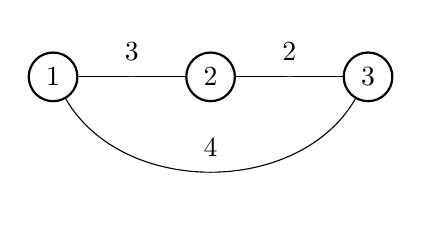
\begin{tikzpicture}
		\begin{scope}[every node/.style={circle,thick,draw}]
			\node (1) at (0,0) {$1$};
			\node (2) at (2,0) {$2$};
			\node (3) at (4,0) {$3$};

		\end{scope}

		\begin{scope}[>={Stealth[black]},
					  every node/.style={fill=white,circle},
					  every edge/.style={draw=black}]
			\path [-] (1) edge node[above] {3} (2);
			\path [-] (2) edge node[above] {2} (3);
			\path [-] (1) edge [bend right=60] node[above] {4} (3);


			%\path [->] (x1b) edge node (x2b);
%			\path [->] (B) edge[bend right=60] node {$1$} (E);
		\end{scope}
		\end{tikzpicture}
	\item [(i)] True. Prim's algorithm only uses the relative weight comparisons of each edge to proceed, negative edges doesn't cause any problems.
	\item [(j)] True. Suppose some MST $T$ does't contain an $r$-path from node $s$ to node $t$, so T contains a path from $s$ to $t$ with some edges having weight $\geq r$, let $e$ be such an edge, if we remove $e$, we end up with a cut where $s$ and $t$ resides in different partitions, we can add some edge in the $r$-path to get a new MST with lighter total weight, so $T$ cannot be a MST.
\end{enumerate}

\section{DPV 5.23}
\begin{enumerate}
	\item [(a)] No update is needed in this case.
	\item [(b)] We can add edge $e$, it will make $T$ contain exactly a cycle. We can use DFS to find the cycle in linear time, delete the heaviest edge along the cycle will produce a new MST $T'$ for the modified graph (By cut property).
	\item [(c)] $T$ is still the MST of the new graph, since the lighter edge is in $T$. $T$ still has the minimum total weight.
	\item [(d)] In this case, we can delete $e$(suppose $e=(u, v)$) from $T$, this will give us $T_1$(contains $u$) and $T_2$(contains $v$), $T_1, T_2$ can be found by DFS starts from $u, v$ respectively after the deletion of $e$. Then we find a lightest edge between nodes in $T_1$ and nodes in $T_2$, add that edge will produce a MST for modified graph.
\end{enumerate}

\section{DPV 5.28}
\begin{enumerate}
	\item Construct a graph with $n$ nodes each denotes a person, and builds an adjacency list of edges using the list of pairs of who know each other. Then calculate the degree of each node.
	\item Repeatedly delete all nodes with degree less than 5 while updating the degrees of neighbor nodes
	\item Suppose the current number of nodes is $N$, then check whether there is a node in the max heap has degree $> N - 5$, if it does, then delete it and update all neighbors' degree.
	\item Repeat 2-3 until no node is deleted.
	\item The remaining nodes denote the people Alice should invite. These people satisfy the two constraints.
\end{enumerate}

This produce the best choice to invite as many people as possible because we starts with inviting everyone. And after that, all people that have less than 5 acquaintances must leave. After one round of step 2. All people remaining have at least 5 known people.

Then we must check the second constraint. We find any person that does not have 5 strangers, he/she must leave. The order really doesn't matter because delete anybody from the invite list cannot increase the number of strangers for each person.


The first step runs in $O(|V|+|E|)$.

This total time running step 2 and 3 is bounded by $O(|V|\cdot|V|)$ (in the worst case, all n people must be deleted from the invited list, it takes $O(|V|)$ to find a node to delete, each deletion causes update to at most $O(|V|)$). Therefore, the algorithm is overall $O(|V|^2) = O(n^2)$.


\section{DPV 5.32}
Simply sort all customer by their service time ascendingly. That is, if for customer $u$ and $v$, if $t_u < t_v$, then we service customer $u$ first.

Suppose that the optimal order is not in sorted order ascendingly, i.e. there exist position $u, v$ in the sequence and $t_u > t_v$. Then the total waiting time is:
\[ T = \sum_{i=1}^{u-1}\sum_{j=1}^i t_j + \sum_{j=1}^u t_j + \sum_{i=u+1}^{v-1}\sum_{j=1}^i t_j + \sum_{j=1}^v t_j + \sum_{i=v+1}^n\sum_{j=1}^i t_j\]

If we swap the service position of $u, v$, we get a new sequence which has the total waiting time:
\[T' = \sum_{i=1}^{u-1}\sum_{j=1}^i t_j + (t_v - t_u + \sum_{j=1}^{u} t_j) + \sum_{i=u+1}^{v-1}(t_v - t_u+ \sum_{j=1}^i t_j) + \sum_{j=1}^v t_j + \sum_{i=v+1}^n\sum_{j=1}^i t_j\]

Note that,
\[T' - T = t_v - t_u + \sum_{i=u+1}^{v-1}(t_v - t_u) < 0\]

Therefore we can always get a more optimal solution by swap any two pairs that's not ordered by their service time, service in ascending order is optimal. The sorting is bound by $O(n\log n)$.

\section{DPV 5.34}
Suppose $n = 2^k$, we number the $n$ elements as $1, 2,...,n$, the base set is $B = \{1, 2, ...,n\}$, other $k+3$ sets are given below:
\begin{align*}
	S_1 &= \{3\} \\
	S_2 &= \{4\} \\
	S_i &= \{2^{i-1}+1, 2^{i-1}+2, ..., 2^i\} , 2 < i < k\\
	S_k &= \{2^{k-1}+1, 2^{k-1}+2, ..., 2^k, 1, 2\}
	S_p &= \{1, 3, 5, ..., 2^k-1\} \\
	S_q &= \{2, 4, 6, ..., 2^k\}
\end{align*}
Note that, for any $0 \leq i, j \leq k, i \neq j, S_i \cap S_j = \emptyset$, and also $\bigcup_{i=0}^k S_i = B, |S_i| = 2^{i-1}, |S_k| = 2^{k-1} + 2, |S_1| = |S_2| = 1, |S_p| = |S_q| = 2^{k-1}$.

The optimal solution for this instance is to choose $S_p$ and $S_q$, only two sets.

Since the greedy algorithm choose the set that covers most elements at each step, it will first pick $S_k$, which covers $2^{k-1} + 2$ elements, after this,

it will choose sets $S_k, S_{k-1}, S_{k-2}, ..., S_3$ in order. Note that at each step, $S_p$ and $S_q$ are at tie with $S_i$, the algorithm will choose $S_i$ to break tie as long as we place $S_p$ and $S_q$ in the right place of the input.

Therefore, for such an instance, the optimal cover uses just two sets, while the greedy algorithm picks at least $k+1$ sets, with $k = \log n$.

In the chapter, a "$<=$" result is achieved (greedy uses at most $k\log n$ sets.), here we get a "$>=$", therefore the approximation ratio we derived is tight.

\section{}
For this algorithm to ouput a MST, I think its edges must have distinct edges. Otherwise, for the following graph, it will produce a cycle.

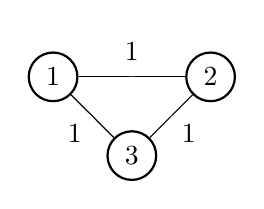
\begin{tikzpicture}
	\begin{scope}[every node/.style={circle,thick,draw}]
		\node (1) at (0,0) {$1$};
		\node (2) at (2,0) {$2$};
		\node (3) at (1,-1) {$3$};

	\end{scope}

	\begin{scope}[>={Stealth[black]},
				  every node/.style={fill=white,circle},
				  every edge/.style={draw=black}]
		\path [-] (1) edge node[above] {1} (2);
		\path [-] (2) edge node[below right] {1} (3);
		\path [-] (1) edge node[below left] {1} (3);
	\end{scope}
	\end{tikzpicture}

\begin{enumerate}
	\item [(a)] Consider the cut of one component (initially just a vertex) and all other components (vertices), according to the cut property, the shortest edge $e$ across the component and other vertices, $T\cup \{e\}$ must be some MST.

	At the end of this algorithm, only one component remains, this is the MST we want.
	\item [(b)]
	Step 1 can be done with DFS in $O(E)$. In step 2, at each iteration, we can use DFS to find all components and also find the lightest edge out of each component, this can be done in $O(E)$.

	Note that, in step 2, each iteration reduces the number of components by half (adding an edge connects two components). So we will do step 2 at most $\log |V|$ times.

	Therefore, this algorithm can run in $O(|E|\log |V|)$.
\end{enumerate}
\end{document}